%\documentclass[10pt, conference, compsocconf]{IEEEtran}
%\documentclass[10pt,journal,cspaper,compsoc]{IEEEtran}
%\documentclass[journal,letterpaper,compsoc,twoside]{IEEEtran}
\documentclass[10pt,journal,compsoc]{IEEEtran}

\usepackage{cite}
\usepackage{graphicx}
\usepackage{psfrag}
\usepackage{subfigure}
\usepackage{url}
\usepackage{color}
\usepackage{balance}
\usepackage[all]{xy}
\usepackage{listings}
\usepackage{array,booktabs,arydshln,xcolor}
\usepackage{tikz}
\usetikzlibrary{shapes,patterns,calc,shapes.geometric,arrows}
\usepackage{makecell}
\usepackage{multirow}
\usepackage{xcolor}
\usepackage{url}
\usepackage{amsthm}
\usepackage{pgfplots}
\usepackage{float}
\usepackage{amsmath}
\usepackage{soul}
\newtheorem{example}{Example}[section]

%\theoremstyle{definition}
%\newtheorem{definition}{Definition}[section]
%\newtheorem{example}{Example}[section]

\begin{document}

\title{Title}

\author{Marco Anisetti~\IEEEmembership{Senior Member,~IEEE,}, Claudio A. Ardagna~\IEEEmembership{Senior Member,~IEEE,} Alessandro Balestrucci, Chiara Braghin, Ernesto Damiani~\IEEEmembership{Senior Member,~IEEE,}, Antongiacomo Polimeno % <-this % stops a space
\IEEEcompsocitemizethanks{\IEEEcompsocthanksitem M. Anisetti, C.A. Ardagna, E. Damiani, are with the Dipartimento di Informatica, Universit\`a degli Studi di Milano, Milano,
Italy. E. Damiani is also with.\protect\\
E-mail: \{firstname.lastname\}@unimi.it
}
\thanks{}}

%\markboth{~}{~}

\IEEEcompsoctitleabstractindextext{%
\begin{abstract}
The conflict between the need of protecting and sharing data is hampering the spread of big data applications. Proper security and privacy assurance is required to protect data owners, while proper data access and sharing are fundamental to implement smart big data solutions. In this context, access control systems assume a central role for balancing the need of data protection and sharing. However, given the software and technological complexity of big data ecosystems, existing solutions are not suitable because they are neither general nor scalable, and do not support a dynamic and collaborative environment. In this paper, we propose an access control system that enforces access to data in a distributed, multi-party big data environment. It is based on data annotations and secure data transformations performed at ingestion time. We show the feasibility of our approach with a case study in a smart city domain using an Apache-based big data engine.

\end{abstract}

\begin{IEEEkeywords}
Access Control, Big Data, Data Transformation, Data Ingestion
\end{IEEEkeywords}}

\maketitle

\IEEEdisplaynotcompsoctitleabstractindextext

\IEEEpeerreviewmaketitle

\section{Introduction}
TBW

\section{Requirements and System Model}

\subsection{System Model}



Abbiamo coalizione di servizio da un lato (ad esempio comuni che offrono servizi alla cittadinanza) e coalizione di utenti (cittadini, security operator) che accedono alla pipeline dall’altro.

Coalizione dove ogni servizio della pipeline è eseguito potenzialmente da utenti e piattaforme differenti. 

Dati potenzialmente condivisi sulla piattaforma in visione Open Data.

Ad ogni passo verso un servizio in coalizione di un utente diverso ci potrebbe essere la necessità di un’ingestion MEDES-style.

NOTA: le pipeline sono completamente instanziate, la variabilità è sull’utente (soggetto) come in medes

NOTA2: perché abbiamo bisogno di AC ad ogni task?
\begin{itemize}
    \item alcuni parametri di configurazione o task da eseguire potrebbero cambiare a seconda della specifica esecuzione, ad esempio scelgo il k attraverso elbow method, oppure ho un processo airflow che contiene alternative e variabili di decisione
    \item in una coalizione un task può essere fornito da provider differenti con dominio di appartenenza diverso e impatto diverso sulla pipeline e sull’AC. Ad esempio, un task fornito dalla corea del nord è a rischio
\end{itemize}


\subsection{2.2 Requirements}
Rivisitazione dei requisiti di MEDES in ottica pipeline, coalizione etc.

\subsection{Reference Scenario}
IMPETUS 


\section{Access Control Policy Language}

\subsection{Access Control Policy}

Il dato annotato (abbiamo applicato Medes in fase di ingestion) arriva a un servizio, il nostro access control component deve prendere una decisione rispetto alla richiesta che possiamo esprimere come: $<$utente, esegui servizio, dato annotato, contesto, trasformazione$>$

\begin{itemize}
    \item esegui servizio è troppo specifico allora dovremmo identificare categorie di servizi a diverse criticità
    \item soluzione marco e chiara andare a basso livello e vedere come vengono trattati i dati (map reduce), claudio lavora ad alto livello ad esempio guardando il tipo di classificazione che si fa (M/F oppure eterosessuale/omossessuale)
    \item altro?
    \item potremmo definire come calcolare o selezionare manualmente la criticità di un servizio istanziato trasformando la politica in
    \item $<$utente, esegui servizio a criticità X, dato annotato, contesto, trasformazione$>$
\end{itemize}


Il dato può essere trasformato a seconda:
\begin{itemize}
    \item tipo e annotazione
    \item utente
    \item criticità del servizio
    \item contesto
\end{itemize}

In certi momenti la trasformazione potrebbe essere deanonimizza, quindi dobbiamo stare attenti all’ordine di applicazione della politica (XACML -$>$ priorità, ad esempio politica emergenza priorità alta quindi fa overwrite delle altre)
\begin{itemize}
    \item $<$utente, esegui servizio a criticità X, dato annotato, contesto, trasformazione, priorità$>$
    \item \textbf{DA DECIDERE SE SERVE LA PRIORITA’ O BASTA SOLO LA POLITICA SENZA ORDINAMENTO (CHIARA/CLAUDIO SI STANNO CONVINCENDO CHE LA PRIORITA’ NON SERVA). IL MOTIVO ORIGINARIO PER CONSIDERARE LA PRIORITA’ ERA}
    \begin{itemize}
        \item DA DECIDERE: se ad ogni connessione S1--$>$S2 applichiamo delle trasformazioni multiple o no? Facciamo prima ingestion medes e poi trasformazione sul servizio o è un passo solo? Il passo multiplo potrebbe essere utile per utenti diversi nella coalizione
        \begin{itemize}
            \item ingestion+servizio
            \item pipeline:  \{servizio ingestion+servizio analitica\}$_n$
        \end{itemize}
    \end{itemize}
\end{itemize}


\subsection{Annotations}
\textbf{Data annotation} presa da MEDES

\textbf{Task annotation:} Come modelliamo la criticità del servizio? (dati in ingresso e tipi del servizio devono essere indipendenti)
\begin{itemize}
    \item Dato annotato in modo indipendente
    \item Servizio ha criticità indipendente dal dato. Possiamo pensare che la criticità dipenda da delle proprietà del servizio che evidenziano relazioni tra input e output esempio Trasparenza e interpretability 
    \item Bisogna differenziare tra predizione (classificazione binaria o più il tipo di classificazione va considerato) e modellazione
    \item task provider
\end{itemize}

\subsection{Data Transformation}
Presa da MEDES e raffinata. Possibili trasformazioni

In certi momenti la trasformazione potrebbe essere deanonimizza, quindi dobbiamo stare attenti all’ordine di applicazione della politica (XACML -$>$ priorità, ad esempio politica emergenza priorità alta quindi fa overwrite delle altre)

\section{Quality vs Privacy}
Definire e modellare metriche quantitative che indichino quanto dato è rimasto rispetto all’originale ingestion time
\begin{itemize}
    \item Sono metriche sui dati manipolati. Ad esempio, numero di feature soppresse, numero di datapoint soppressi. Queste due potrebbero essere pesate su feature ranking.
\end{itemize}

\section{Coalition Building}
Data lineage is a set of complex relationships between datasets an jobs in a pipeline. 
The scope of this paper is to add control on the data lineage differentiating data flow from processing pipeline and controlling them separately: i) data controlled using AC and transformations prior to be feed into a processing jobs, ii) processing controlled selecting the suitable processing jobs among a set of available and compatible alternatives offered by different service provider S.

\begin{figure}[!t]
	\centering
	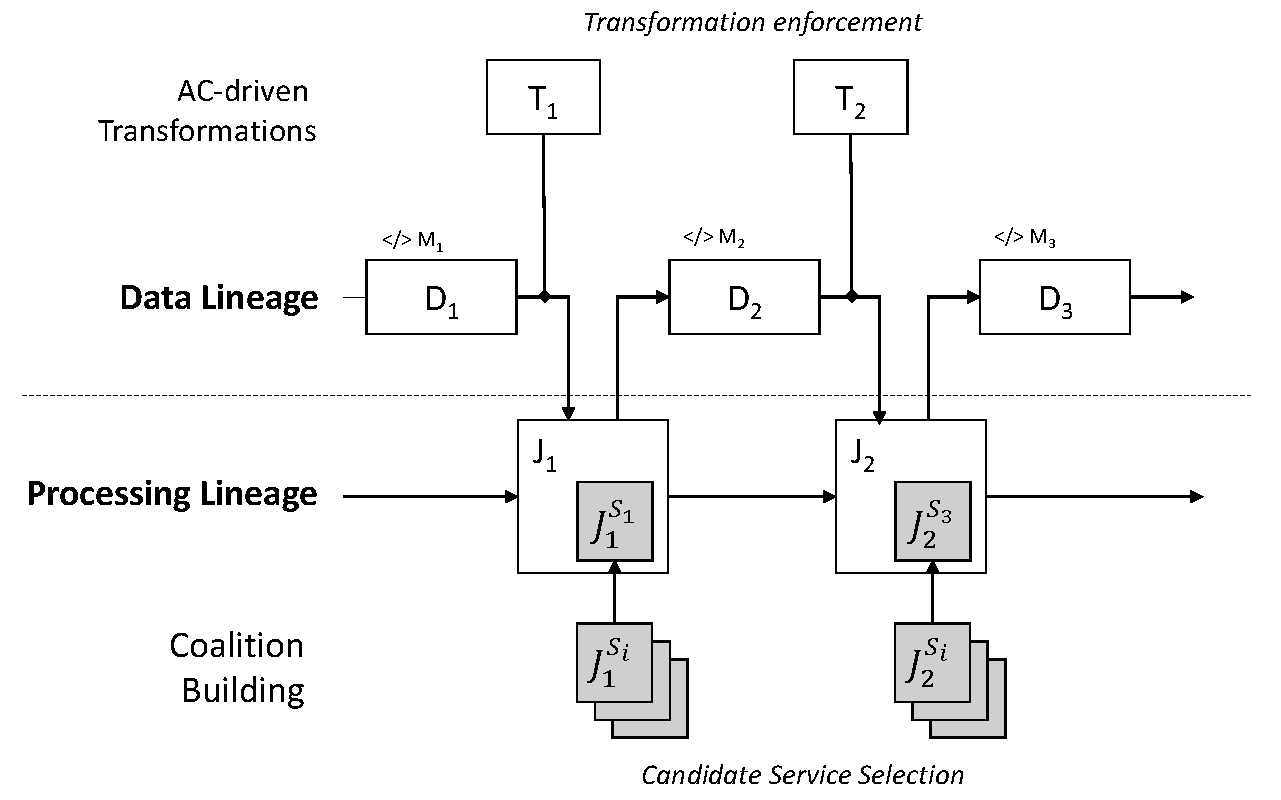
\includegraphics[width=0.48\textwidth]{meth.pdf}
\caption{Methodology.}
	\label{fig:smet}
\end{figure} 

In this paper, for the sake of simplicity we assume that the transformation on the data made by the processing jobs are known and not influenced by the service provider behaviour, trusting the service provider to produce the correct transformation requested by the given job.
With this assumption the coalition selection is assumed to be equivalent to select different service provides for the different jobs and thus different transformation policies to be applied on the data.

\begin{example}\label{ex:p1j}
Let us consider the following example where we have a pipeline made of just one ingestion job that can be offered by service provider $s_1$ or by the service provider $s_2$. In case the $s_1$ is selected the transformation $T_1$ is triggered according to the authorization $s_1$ has on the data, in this example $s_1$ has full control meaning that transformation $t_1$ is empty. In case the $s_2$ is selected the transformation $T_2$ is triggered according to the authorization $s_2$ has on the data and in this example data labelled as PII are removed. 
\end{example}
Considering the two data lineage generated by the two different coalition in Example\ref{ex:p1j} the one involving $s_2$ produce a significant changes to data compared to the other one. This data changes can have direct impact on the quality of the analytics outcomes, therefore our goal is to build coalitions ensuring specific data quality. This coalition building problem can be assimilated to xxx showing an exponential complexity ...
In the following we fist introduce our data quality metrics and then our euristics to solve the problem of coalition building

\subsection{Data Quality metrics}
\subsection{Coalition Heuristics}






Execute a template where for each task a set of functionally equivalent alternatives provided by different service are available.


Con la coalizione, vogliamo mettere per ogni nodo della pipeline servizi equivalenti forniti da utenti diversi e tra cui scegliere? Se sì, definire le euristiche per la selezione con identificazione del servizio a qualità maggiore.
\begin{itemize}
    \item come calcolare la qualità al punto 1? Vedi sezione 4.
    \item in ogni caso l’indicatore di qualità serve anche se non vogliamo scegliere il servizio ottimo e non abbiamo alternative. Modella un parametro importante del nostro AC. Ad esempio se abbiamo trasformazioni alternative
\end{itemize}

\section{Architectural Deployment}
Parliamo dei due tipi di deployment

COMMENTO (architectural deployment): noi stiamo ragionando usando una coreografia, autocrmap ragionava usando una orchestrazione con un’entità centrale che forniva sandboxing, come se noi avessimo il nostro approccio centralizzato e i servizi vengono di volta in volta a prendersi il dato

\section{Experiments}

\section{Related Work}

\section{Conclusions}
DISCUTERE CON MARCO POSSIBILI ANALOGIE SECURESCM: ad esempio i servizi non sono alternativi ma sono delle piccole coalizioni a loro volta.

(ri)Vedere anche Autocrmap per vedere analogie.

\bibliographystyle{ACM-Reference-Format}
\bibliography{access_control_big_data,varie}

\end{document}

\section{Metriche di qualità vs privacy}
\begin{itemize}
    \item quanto l'applicazione delle tecniche di AC cambia il dataset o i dataset
    \item ad esempio parametri quantitativi sul dataset (cardinalitùà)
    \item parametri statistici del dataset
    \item pensieri di Ernesto
    \begin{itemize}
        \item In sede di ingestion, la valutazione sull’impatto dell’analitica la posso fare. Se privacy e valori numerici si può compiare epsilon e delta di differential privacy (noise addition o allargare la distribuzione di rumore sulla base del budget di privacy). 
        \item Metriche quantitative, come ricercar potrebbe essere interessante schema di budget di privacy per l’offuscamento di dati non numerici Quante volte il dato viene trasformato
        \item Analitiche di statistica descrittiva per il 3sigma -> piattaforma di puliafito (Catania)
        \item Anomaly detection con deviazione standard
        \item Data sanitizzato fa il merge di due barre dell’istogramma è un’autoencoding, come cambia la deviazione standard
    \end{itemize}
\end{itemize}

\section{Experiments}
Contattare PD
